\documentclass[polish,polish,a4paper,11pt]{article}

\usepackage{babel}
 \usepackage{pslatex}
\usepackage[utf8]{inputenc}
\usepackage{polski}
\usepackage{graphicx} 
 \usepackage{amsmath}
  \usepackage{geometry}
  \geometry{a4paper, total={170mm,257mm}, 
   left=30mm,
   right=20mm,
   top=25mm,
   bottom=25mm}
  \setlength{\parindent}{4em}
   \setlength{\parskip}{1em}
 \usepackage{fancyhdr}
 \usepackage{enumerate}
 
\title{Sprawozdanie \\Ćwiczenie komputerowe z dynamiki molekularnej}
\author{Jakub Sobolewski \\ 274437}
\begin{document}
\maketitle

\newcounter{Rys}
\section{Opis oprogramowania}
\begin{itemize}
\item Do wykonania symulacji wykorzystano język C++11
\item Wizualizacja została wykonana w OpenGL
\item Wykresy zostały stworzone z pomocą języka Python i biblioteki Matplotlib
\end{itemize}
\subsection{Struktura programu}
\begin{itemize}
\item $main.cpp$ - główna funkcja programu
\item $GasSimulation.h$ - biblioteka implementująca wszystkie wymagane symulacje
\item $Utils.h$ - biblioteka implementująca trójwymiarowy wektor, wektor bazowy, oraz szybszą funkcję do obliczania potęgi z wykładnikiem naturalnym dodatnim od funkcji z bibioteki standardowej $std::pow()$
\item $plot.py$ - skrypt rysujący wykresy
\end{itemize}

\subsection{Stabilność rozwiązania}
\begin{center}
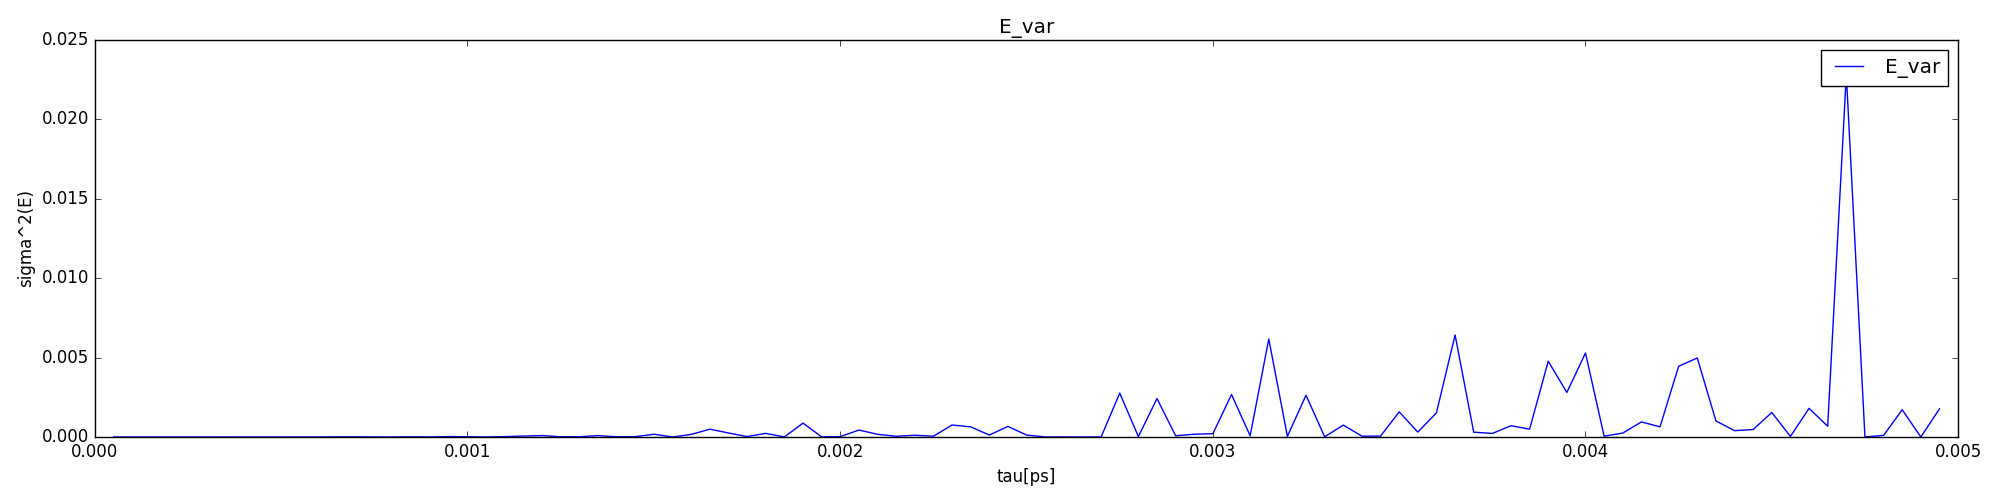
\includegraphics[scale=0.3]{../Data/E_var.png}
\end{center}
\stepcounter{Rys}
\begin{center}
Rys. \arabic{Rys} Wariancja energii w funkcji kroku czasowego $\tau$.
\end{center}
Widać że dla kroku mniejszego niż 0.001ps symulacja jest stabilna.
 
\subsection{Minimum energii kryształu}
\begin{center}
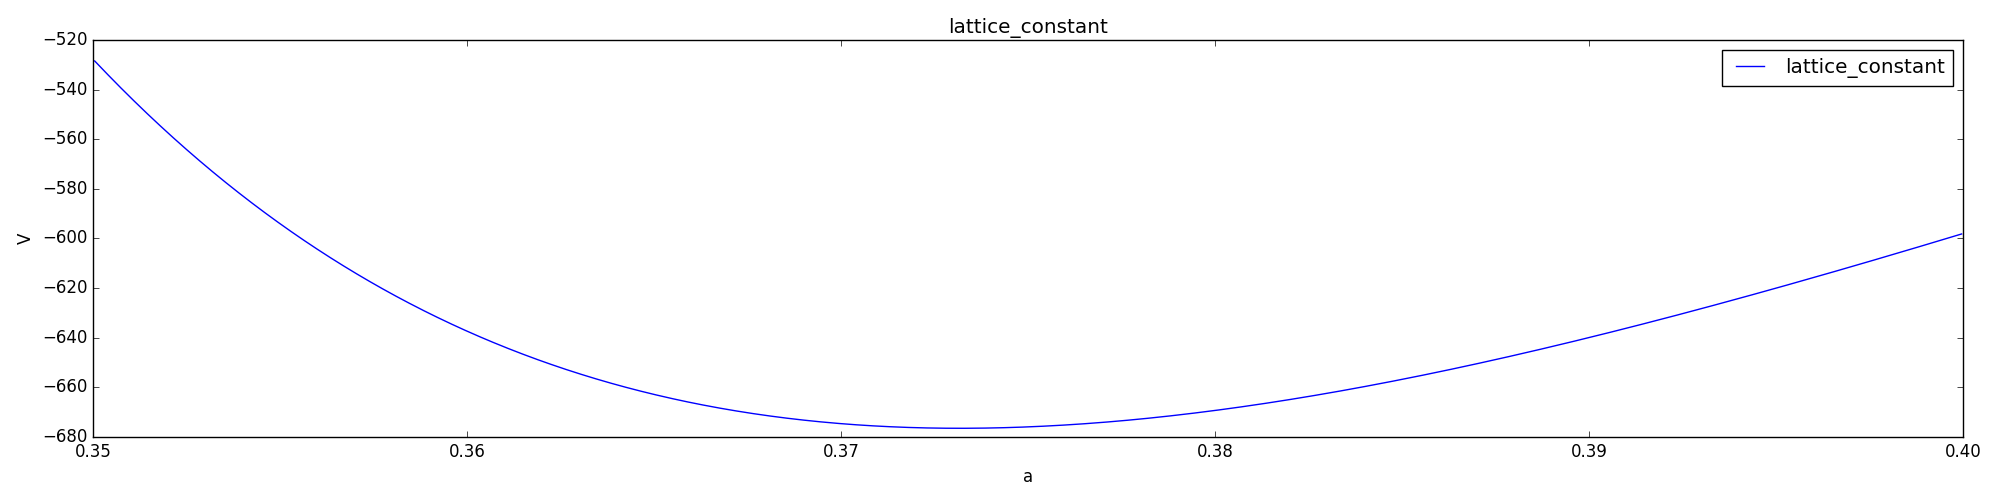
\includegraphics[scale=0.3]{../Data/lattice_constant.png}
\end{center}
\stepcounter{Rys}
\begin{center}
Rys. \arabic{Rys} Wykres energii potencjalnej kryształu w funkcji stałej kryształu.
\end{center}
Dla stałej siatki równej $a=0.372um$ kryształ znajduje się w minimum energii w temperaturze 0K. 

Temperatura układu w trakcie trwania symulacji wzrasta, jest to spowodowane działaniem niezrównoważonych sił na atomy co przyczynia sie do ich ruchu.
 
\subsection{Zachowanie temperatury i ciśnienia gazu}
\begin{center}
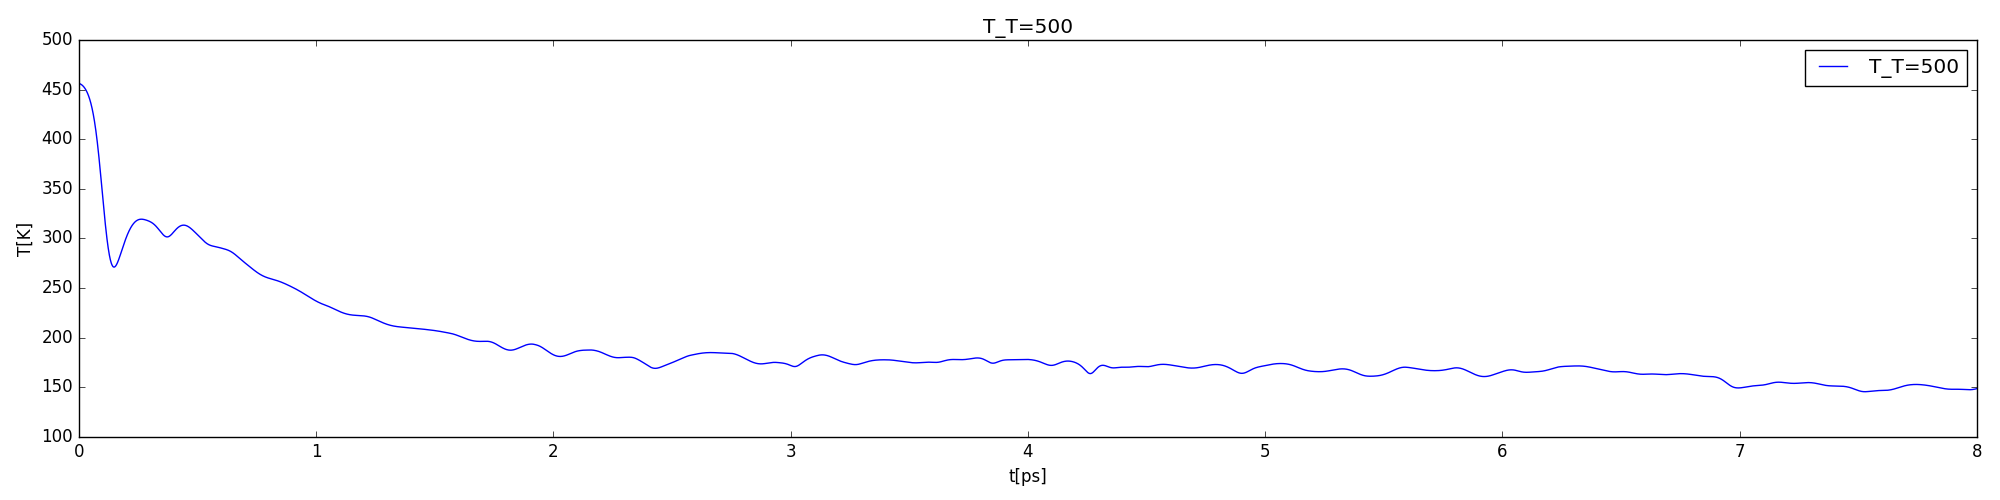
\includegraphics[scale=0.3]{../Data/T_T=500.png}
\end{center}
\stepcounter{Rys}
\begin{center}
Rys. \arabic{Rys} Wykres funkcji temperatury od czasu, $T_0 = 500K$.
\end{center}
\begin{center}
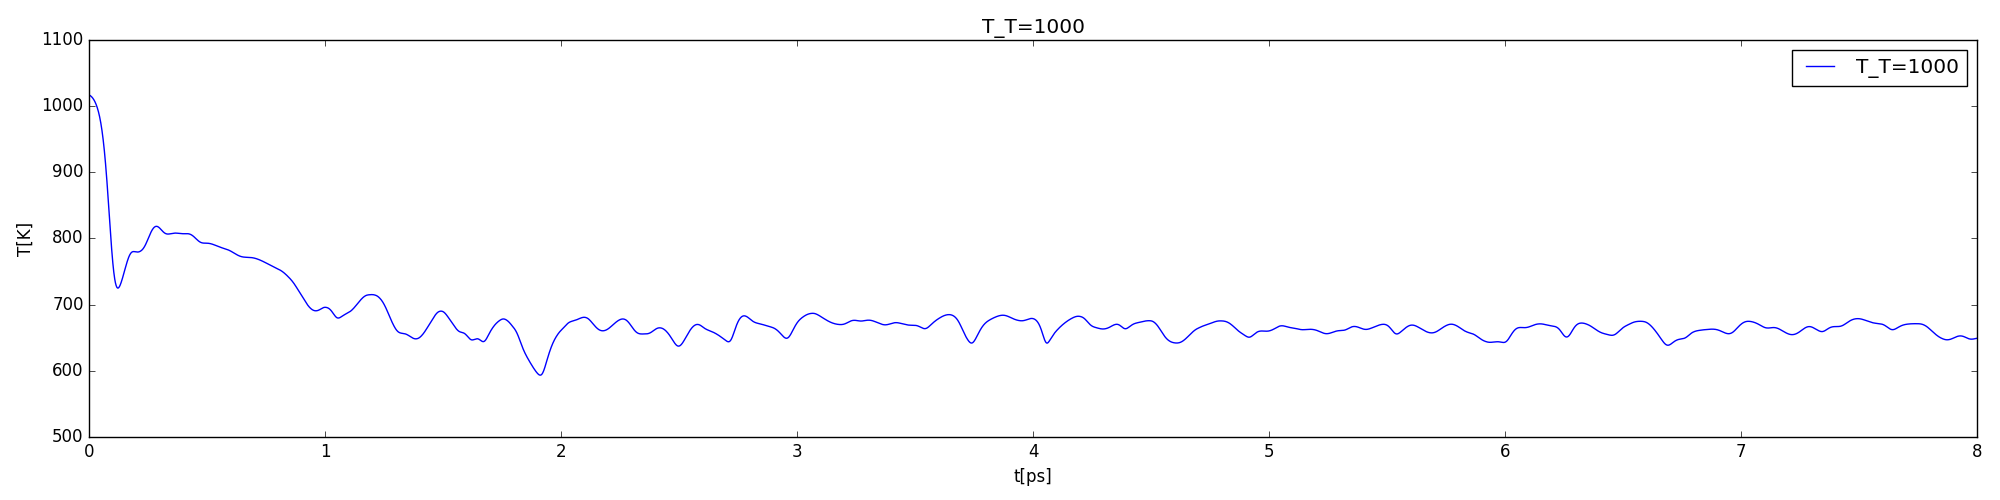
\includegraphics[scale=0.3]{../Data/T_T=1000.png}
\end{center}
\stepcounter{Rys}
\begin{center}
Rys. \arabic{Rys} Wykres funkcji temperatury od czasu, $T_0 = 1000K$.
\end{center}
\begin{center}
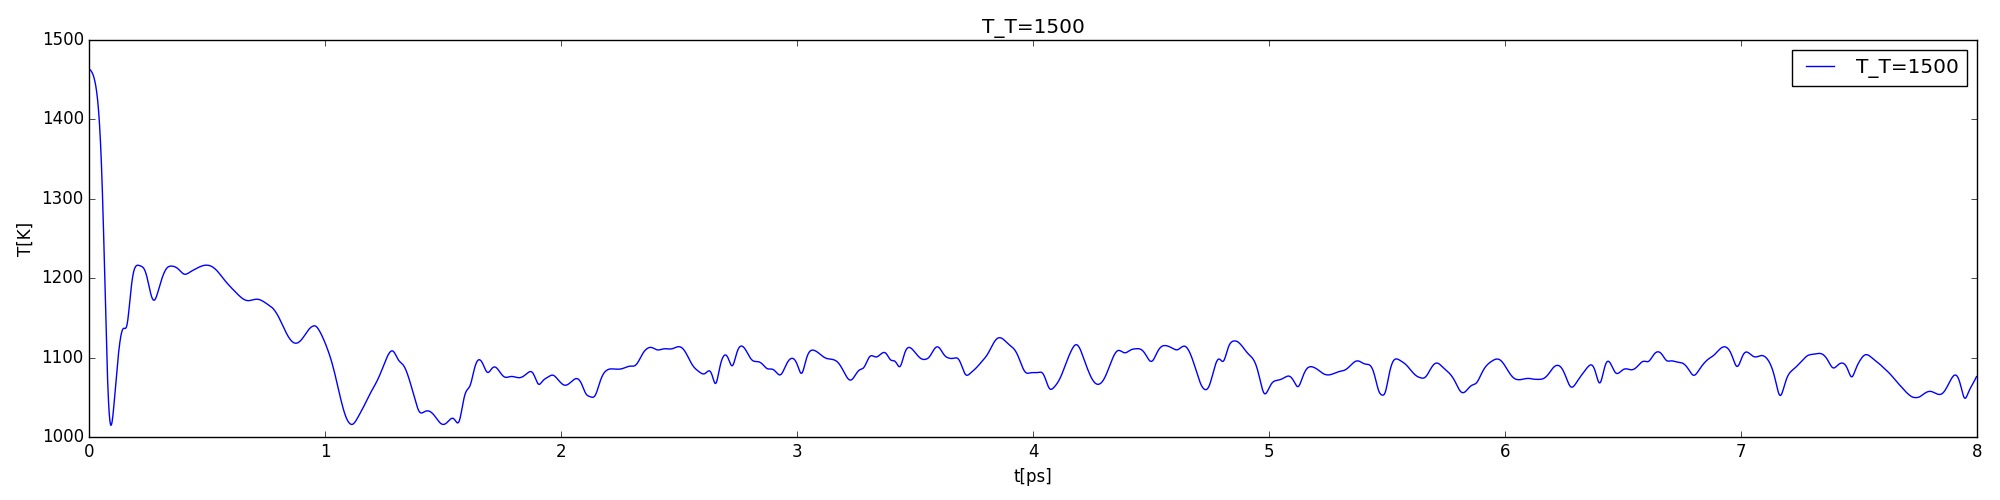
\includegraphics[scale=0.3]{../Data/T_T=1500.png}
\end{center}
\stepcounter{Rys}
\begin{center}
Rys. \arabic{Rys} Wykres funkcji temperatury od czasu, $T_0 = 1500K$.
\end{center}
\begin{center}
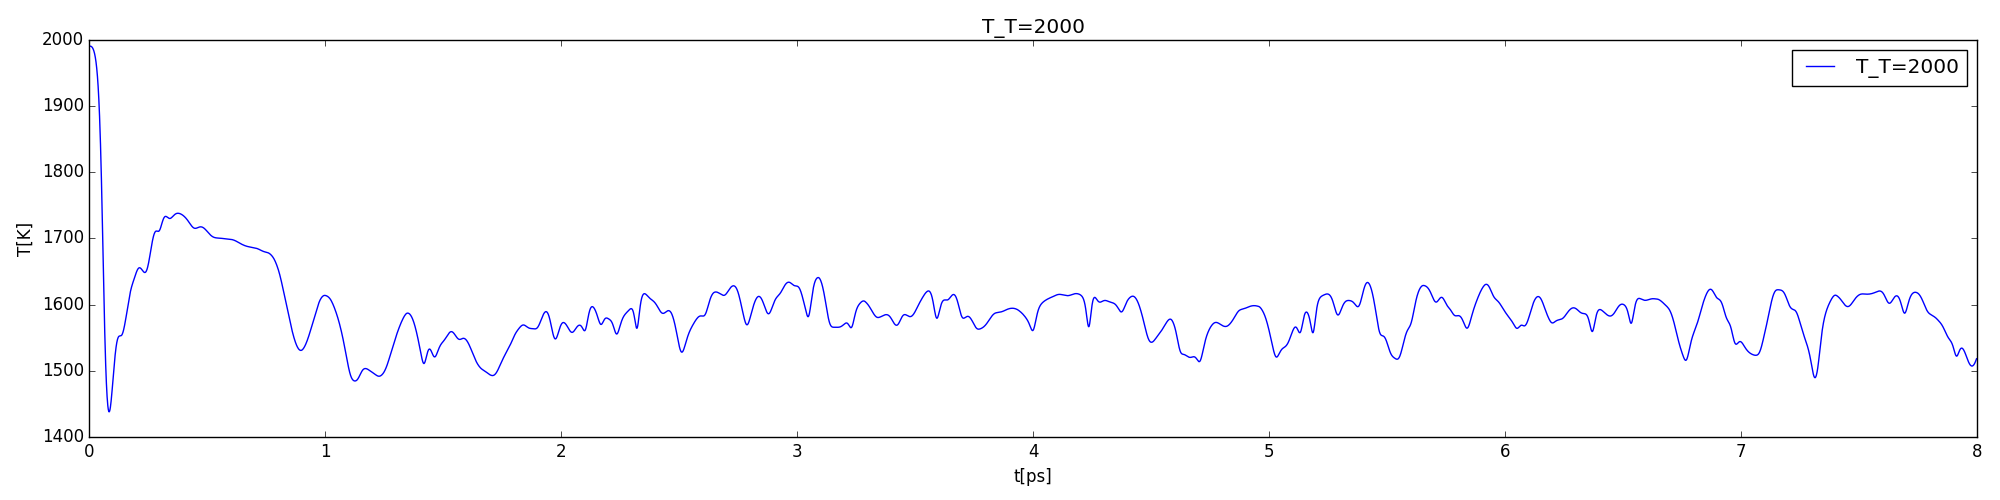
\includegraphics[scale=0.3]{../Data/T_T=2000.png}
\end{center}
\stepcounter{Rys}
\begin{center}
Rys. \arabic{Rys} Wykres funkcji temperatury od czasu, $T_0 = 2000K$.
\end{center}
 
\begin{center}
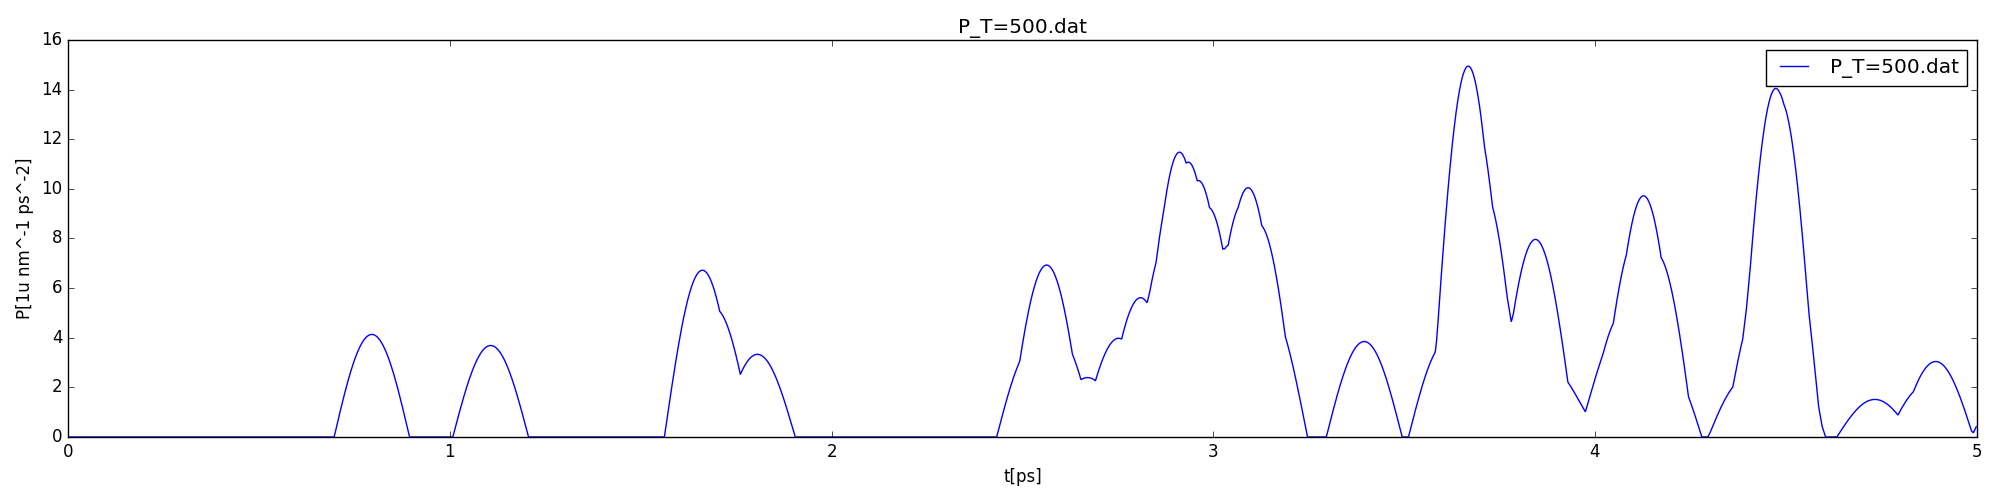
\includegraphics[scale=0.3]{../Data/P_T=500.png}
\end{center}
\stepcounter{Rys}
\begin{center}
Rys. \arabic{Rys} Wykres funkcji ciśnienia od czasu, $T_0 = 500K$.
\end{center}
\begin{center}
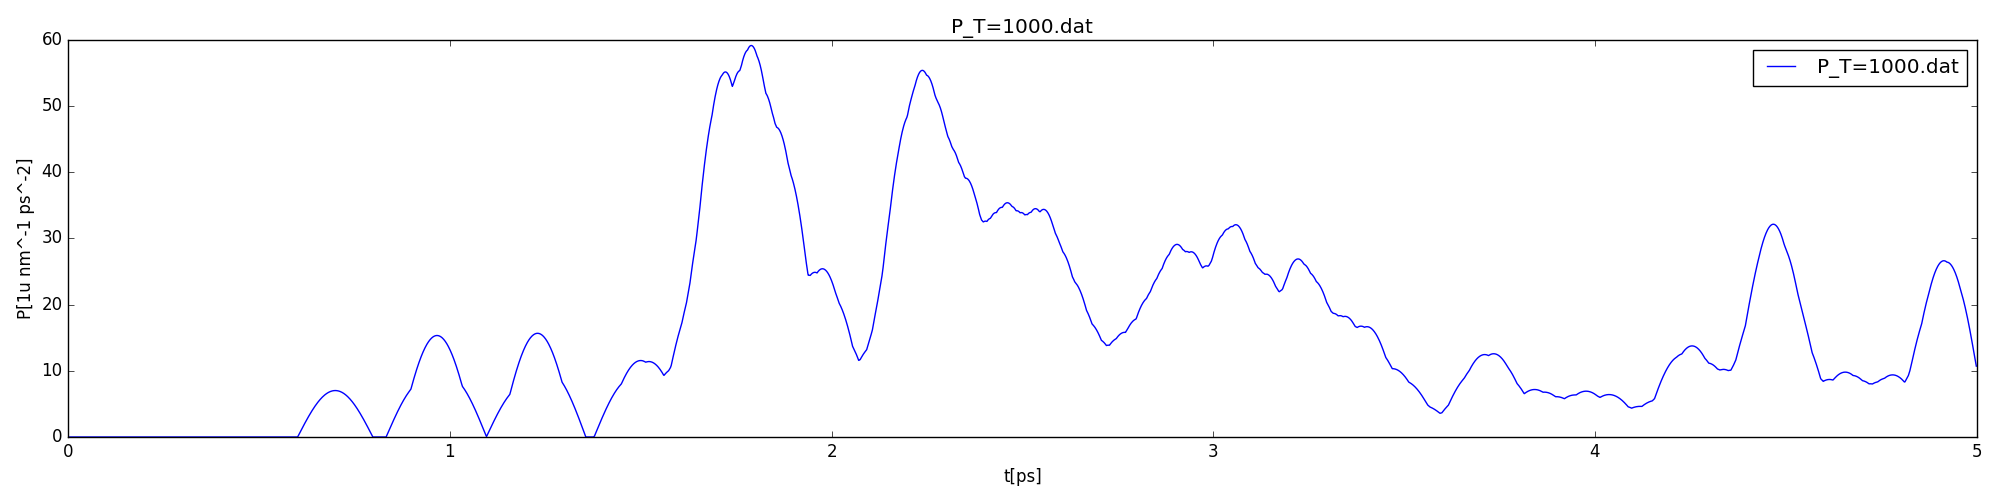
\includegraphics[scale=0.3]{../Data/P_T=1000.png}
\end{center}
\stepcounter{Rys}
\begin{center}
Rys. \arabic{Rys} Wykres funkcji ciśnienia od czasu, $T_0 = 1000K$.
\end{center}
\begin{center}
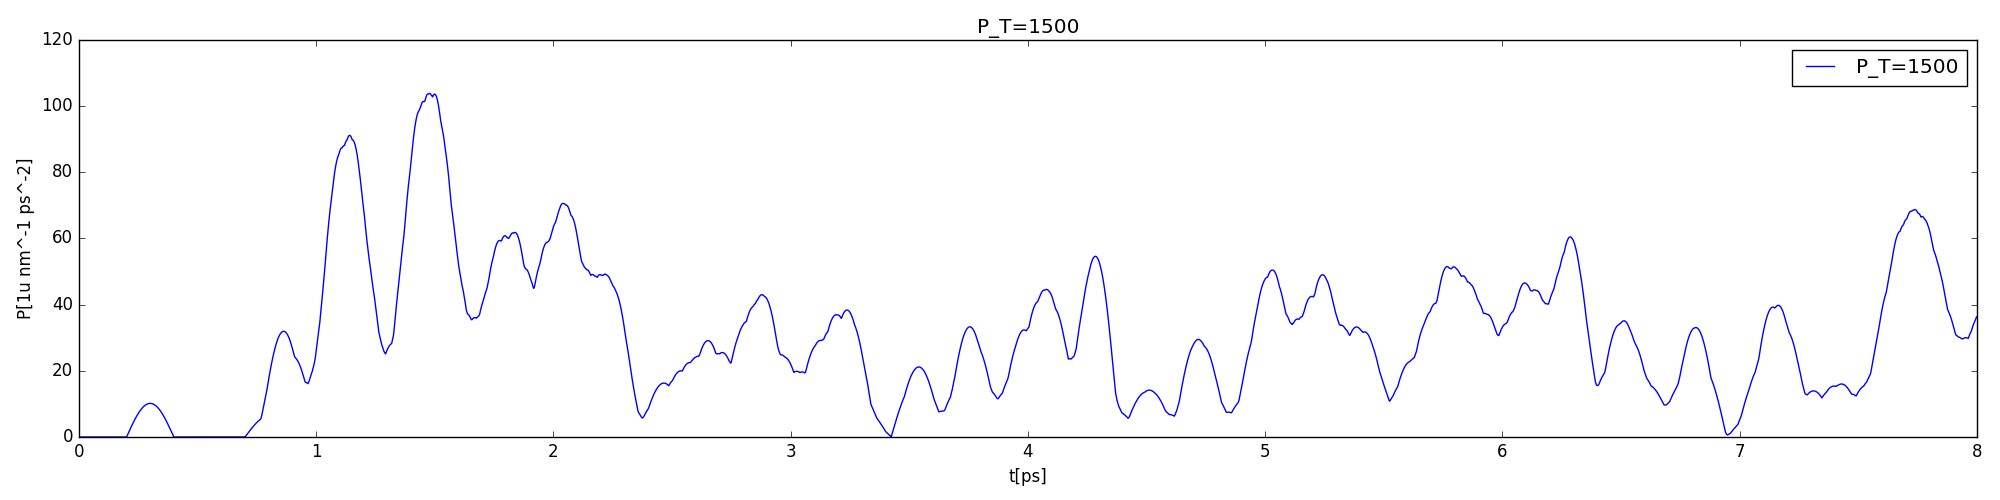
\includegraphics[scale=0.3]{../Data/P_T=1500.png}
\end{center}
\stepcounter{Rys}
\begin{center}
Rys. \arabic{Rys} Wykres funkcji ciśnienia od czasu, $T_0 = 1500K$.
\end{center}
\begin{center}
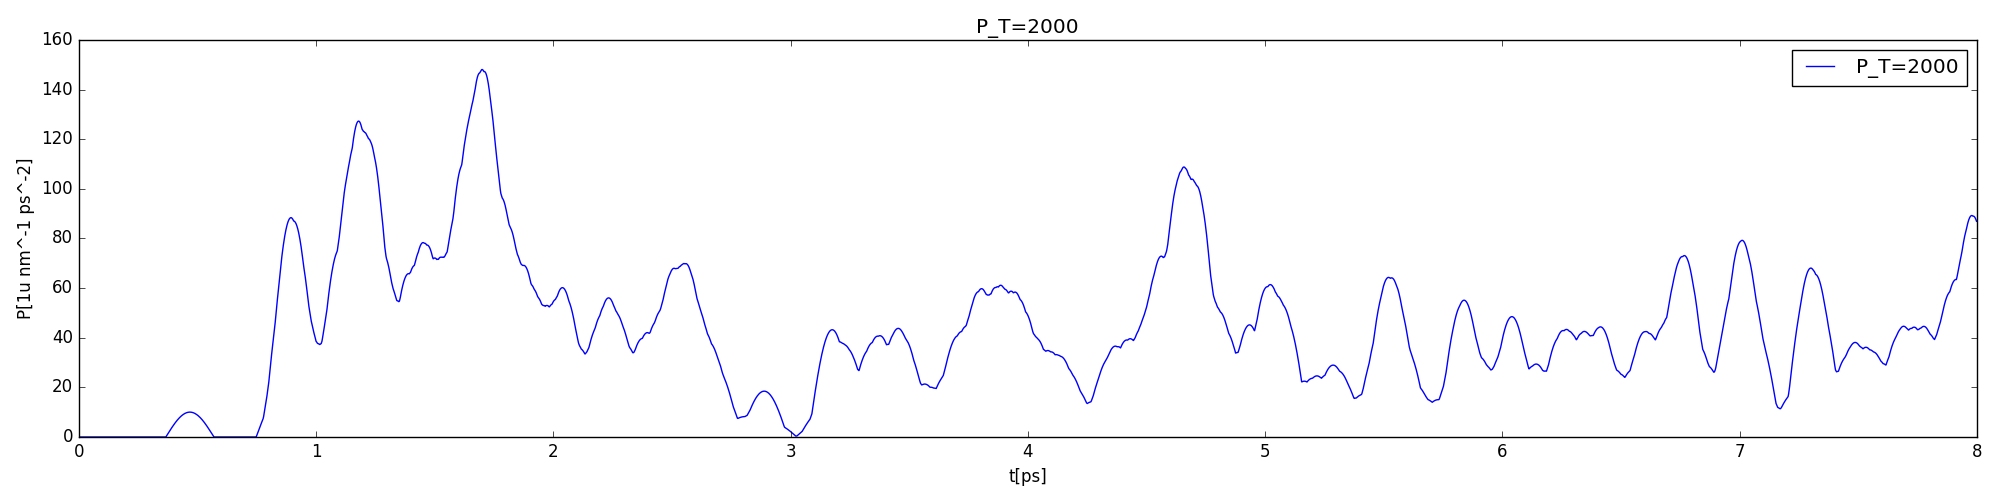
\includegraphics[scale=0.3]{../Data/P_T=2000.png}
\end{center}
\stepcounter{Rys}
\begin{center}
Rys. \arabic{Rys} Wykres funkcji ciśnienia od czasu, $T_0 = 2000K$.
\end{center}

\end{document}